\documentclass[aspectratio=169]{beamer}

% because we need to claim weird things
\newtheorem{claim}{Claim}
\newtheorem{defn}{Definition}
%\newtheorem{lemma}{Lemma}
\newtheorem{thm}{Theorem}
\newtheorem{vita}{Vit\ae}
\newtheorem{qotd}{Quote of the Day}

\usepackage{algorithm}
\usepackage{algpseudocode}
\usepackage{graphics}
\usepackage{ulem}
\bibliographystyle{unsrt}

% background image
\usebackgroundtemplate%
{%
    
\includegraphics[width=\paperwidth,height=\paperheight]{../artifacts/stemulus.pdf}%
}
\setbeamertemplate{caption}[numbered]

% page numbers
\addtobeamertemplate{navigation symbols}{}{%
    \usebeamerfont{footline}%
    \usebeamercolor[fg]{footline}%
    \hspace{1em}%
    \insertframenumber/\inserttotalframenumber
}

% presentation header
\usetheme{Warsaw}
\title{Web Architecture}
\author{Dylan Lane McDonald}
\institute{CNM STEMulus Center\\Web Development with PHP}
\date{\today}

\begin{document}
\begin{frame}
\titlepage
\end{frame}

\begin{frame}
\frametitle{Outline}
\tableofcontents
\end{frame}

\section{Client/Server Model}
\begin{frame}
\frametitle{Client/Server Model}
The client/server model is a classic model that describes multiple small nodes (clients) connecting to and utilizing a centralized node (server). The key idea of the client/server model is all the data is the same no matter what type of client is utilizing the server.

\begin{figure}
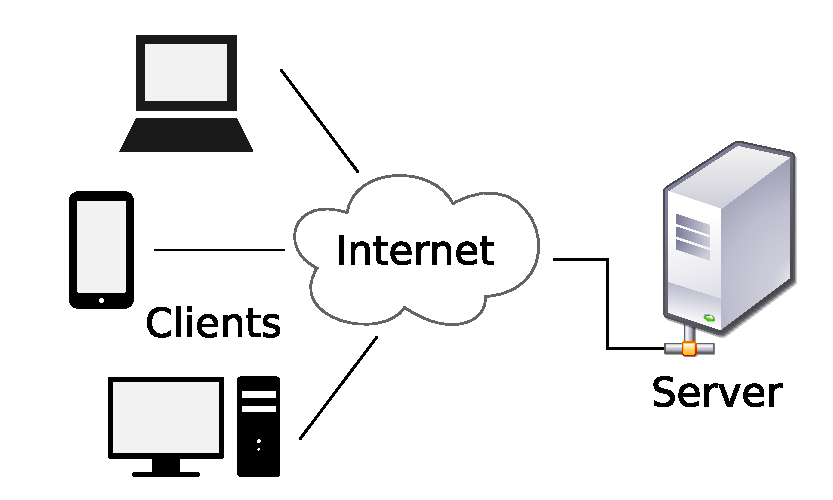
\includegraphics[scale=0.4]{../artifacts/client-server.pdf}
\caption{Client/Server Model}
\label{fig:client-server}
\end{figure}
\end{frame}

\subsection{Client}
\begin{frame}
\frametitle{Client}
In terms of the web, the client is a \textbf{web browser}. A web browser consists of three major components:
\begin{itemize}
	\item \textbf{HTML Renderer}: Responsible for interpreting HTML code and determining where elements are placed on a page and how they show up
	\item \textbf{CSS Layout Engine}: Responsible for interpreting CSS and applying specified styles to the matched HTML elements
	\item \textbf{JavaScript Engine}: Responsible for interpreting JavaScript and executing JavaScript in response to client side events
\end{itemize}
\begin{figure}
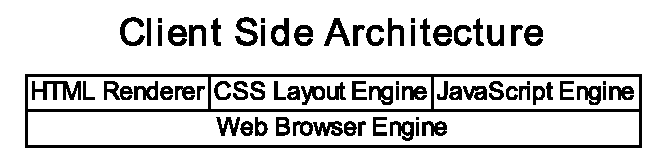
\includegraphics[scale=0.5]{../artifacts/client.pdf}
\caption{Client Side Architecture}
\label{fig:client}
\end{figure}
\end{frame}

\subsection{Server}
\begin{frame}
\frametitle{Server}
The server is a machine configured with multiple \textbf{d\ae mons}\footnote{Windows Server calls these \textbf{services}}, processes that run in an infinite loop replying to incoming requests from clients. Servers typically have very robust CPU, disk, and network configurations. This allows servers to do the ``heavy lifting'' on behalf on clients.

\mbox{}\\
In this class, we will concentrate on the $x$AMP architecture.

\begin{figure}
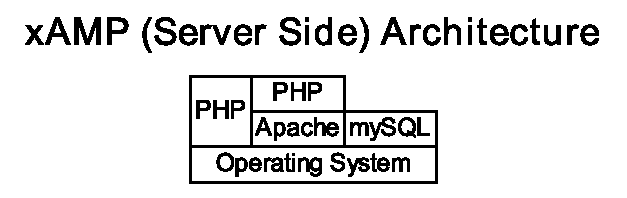
\includegraphics[scale=0.65]{../artifacts/xamp.pdf}
\caption{Server Side Architecture}
\label{fig:server}
\end{figure}
\end{frame}

\section{$x$AMP Stack}
\subsection{What Is it?}
\begin{frame}
\frametitle{What Is The $x$AMP Stack?}
As previously discussed, the $x$AMP stack is the combination of:
\begin{itemize}
	\item \textbf{A}pache
	\item \textbf{m}ySQL
	\item \textbf{P}HP
\end{itemize}

\pause
The word ``stack'' is a computer science term for data layered one upon the other. The name implies that $x$ (the operating system) is the lower layer, the next layer is Apache, the following layer is mySQL, and the last layer is PHP. This is mostly true. One cannot exist without the layer below it.
\end{frame}

\subsection{Operating Systems}
\begin{frame}
\frametitle{Operating Systems}
The lowest layer of the stack is the operating system. The most common operating systems used are:
\begin{itemize}
	\item ``UNIX''?
	\begin{itemize}
		\item Linux\footnote{Linux is \textbf{technically} not UNIX. It's a UNIX clone.}
		\item BSD
		\item Solaris
	\end{itemize}
	\item Mac OS X\footnote{Actually, Mac OS X is more UNIX than Linux is.}
	\item Windows
\end{itemize}
No matter what the operating system, as long as the other components are installable, one can create an $x$AMP stack.
\end{frame}

\subsection{Apache}
\begin{frame}
\frametitle{Apache Web Server}
The Apache web server is the most popular web server today, with a 38\% market share. \cite{netcraft} The name Apache is derived from the myriad of ``patches'' needed to improve its predecessor, NCSA \texttt{httpd} to fix bugs and extend features. Within a year, it became the internet's most popular web server. \cite{apache}

\pause
\mbox{}\\
The purpose of the Apache web server is to listen on the HTTP port (port 80) and receive and reply to HTTP commands such as, ``give me the page \texttt{index.php}'' or ``Take this data and give it to the page \texttt{form\_process.php}''.
\end{frame}

\subsection{mySQL}
\begin{frame}
\frametitle{mySQL}
mySQL is a \textbf{R}elational \textbf{D}atabase \textbf{M}anagement \textbf{S}ystem (RDBMS) is is ``officially pronounced `My Ess Que Ell' (not `my sequel')''. \cite{mysql} mySQL and PostgreSQL are the two most popular open source RDMBSes.

\mbox{}\\
The reference version of mySQL is 5.6. The differences in the 5.$x$ versions of mySQL, while not trivial, are smaller when compared in the version differences in PHP.
\end{frame}

\subsection{PHP}
\begin{frame}
\frametitle{PHP}
PHP (\textbf{P}HP \textbf{H}ypertext \textbf{P}rocessor) is a server side scripting language that has evolved into a larger general purpose programming language. The current version is 7. PHP remained at 5.$x$ for 11 years and PHP 5.$x$ code, especially PHP 5.5 and 5.6 code are still in active use.

\mbox{}\\
PHP is a highly extensible language with multiple extensions installable server wide. In addition, individual projects can be extended by using \texttt{*.phar} files (a mnemonic for ``PHP archive'') without the necessity of deploying system wide changes to the PHP configuration. The \href{https://getcomposer.org/}{Compser}\footnote{Composer is akin to Java's Maven} project also allows one to add additional features to PHP without deploying system wide changes to the PHP configuration.
\end{frame}

\section{Open Source}
\begin{frame}
\frametitle{Open Source}
All the components of the $x$AMP stack, as well as some of the possible operating systems are open source.
\pause
\begin{qotd}
``When I released GNU Emacs and people started using it, they started sending me improvements in the mail. So I would get a message with a bug fix, and a message with a new feature, and another bug fix, and another new feature, and another... and another... until they were pouring in on me so fast that just taking advantage of all of the help people were giving me was a big job. Microsoft doesn't have this problem.''\\
$\approx$ Richard Stallman
\end{qotd}
\end{frame}

\begin{frame}
\frametitle{Open Source}
The open source movement was, among other people, started by Richard Stallman when he worked at the artificial intelligence lab at MIT in the 1970s.
\pause
\begin{vita}
\textbf{Richard Stallman} is the founder of the GNU Project and Free Software Foundation. He also pioneered the ``copyleft'' movement to legally protect free software. He remains a visible (and somewhat controversial) figure in the software industry and dedicates his life to the free software movement.
\end{vita}
\end{frame}

\section{HTTP Conversation}
\begin{frame}
\label{slide:conversation}
\frametitle{HTTP Conversation}
Informally, everything on the web happens in an \textbf{HTTP Conversation}. This conversation is typically initiated by the client and consists of one or more replies from the server. Extending the conversation metaphor, such a conversation consists of the following steps:
\begin{itemize}
	\item \textbf{Client}: Hi, server! I need to get \texttt{foo.php}.
	\item \textbf{Server}: Hi, client! Here's \texttt{foo.php}. Can I get anything else for you?
	\item \textbf{Client}: Yes, \texttt{bar.php}.
	\item \textbf{Server}: Here's \texttt{bar.php}. Can I get anything else for you?
	\item \textbf{Client}: No thank you. Goodbye.
\end{itemize}
The conversation will continue until the client has requested all the items required.
\end{frame}

\begin{frame}
\frametitle{HTTP Request}
\begin{figure}
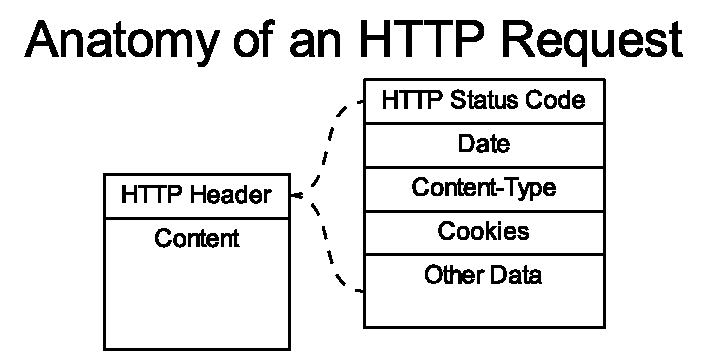
\includegraphics[scale=0.85]{../artifacts/http-request.pdf}
\caption{HTTP Request}
\label{fig:http-request}
\end{figure}
\end{frame}

\begin{frame}
\frametitle{HTTP Request}
Figure \ref{fig:http-request} depicts the anatomy of the conversation outlined in Slide \ref{slide:conversation}. Notice there are two slices of the reply from the server: the header and the content. The \textbf{header} contains the metadata\footnote{``data about data''} about the request.

\mbox{}\\
The header contains a lot about the request. Of particular interest in the header is:
\begin{itemize}
	\item \textbf{HTTP Status Code}: a 3 digit code that indicates the result:
	\begin{itemize}
		\item 1XX: incomplete, but not yet failed
		\item 2XX: complete, successful
		\item 3XX: complete, somewhere else
		\item 4XX: error, blame the client
		\item 5XX: error, blame the server
	\end{itemize}
	\item \textbf{Content Type}: what type of data the request produced
\end{itemize}
\end{frame}

\begin{frame}
\frametitle{Static HTTP Conversation}
Returning to the conversation in Slide \ref{slide:conversation}, what if the server doesn't need to conduct database queries, contact other servers, etc and is able to grab all content internally? This is a known as a \textbf{static use case}. A static use case would sound something like this:
\begin{itemize}
	\item \textbf{Client}: Hi, server! I need to get \texttt{static.php}.
	\item \textbf{Server}: Hi, client! Here's \texttt{static.php}. Can I get anything else for you?
	\item \textbf{Client}: No thank you. Goodbye.
\end{itemize}
Notice no extra steps are required by the server in the static use case.
\end{frame}

\begin{frame}
\frametitle{Dynamic HTTP Conversation}
Now suppose the server does need to conduct database queries, contact other servers, etc and some content relies on external data. This is a known as a \textbf{dynamic use case}. A dynamic use case would sound something like this:
\begin{itemize}
	\item \textbf{Client}: Hi, server! I need to get \texttt{dynamic.php}.
	\item \textbf{Server}: Hi, client! One moment while I search my database and contact my partners\dots
	\item \textbf{Server}: \dots thanks for waiting for me to gather external data. Here's \texttt{dynamic.php}. Can I get anything else for you?
	\item \textbf{Client}: No thank you. Goodbye.
\end{itemize}
Notice the server has to delay and wait for the external data to become available in the dynamic use case.
\end{frame}

\begin{frame}
\frametitle{Works Cited}
\bibliography{architecture}
\end{frame}

\end{document}
